
\begin{abstract}
Evaluating probabilistic forecasts is complex and essential across various domains, yet no comprehensive software framework exists to simplify this task. Despite extensive literature on evaluation methodologies, current practices are fragmented and often lack reproducibility. To address this gap, we introduce a reproducible experimental workflow for evaluating probabilistic forecasting algorithms using the sktime package.

The framework includes a unified software API for forecasting algorithms, with a simple specification language for complex forecasting algorithms, including meta-algorithms such as bootstrapping, probabilistic performance metrics, and standardized workflows for evaluation.

We demonstrate the framework's efficacy through a study evaluating prediction intervals added to point forecasts. Our results also highlight the improved prediction accuracy and reliability of combined approaches. We provide reusable code and invite contributions from the research community to extend our experiments and address computational challenges for broader studies.
\end{abstract}

\section{Introduction}

Making probabilistic forecasts is hard - and evaluating probabilistic forecasts, or the algorithms that produce them, is strictly harder.

An entire field of literature is concerned with developing solid meta-methodology for evaluation, including evaluation metrics such as CRPS (cite) and their properties such as properness, benchmarking setups and competitions such as the Makridakis competitions (cite). This meta-field is based on an even larger primary field of methodology development for algorithms producing probabilistic forecasts, spanning classical methods, uncertainty estimation techniques such as bootstrap or conformal intervals, or modern deep learning and foundation models.

Despite the critical relevance of evaluating probabilistic forecasts in many domains, including finance, energy, health care, and climate science, no software framework or interface design has emerged that would cover all of the above with a simple workflow or specification language. For example, the reproducing code for the M competitions - while comprehensive in scope - is based off forecasts that have to be manually generated from non-unified software interfaces. Similar statements are true for other benchmarking studies, if code is available, and often code is not available. This makes it especially difficult for practitioners in industry and academia alike to add to the growing body of evidence, or verify it.

To address these limitations, we present an simple, reproducible experimental workflow for evaluating probabilistic forecasting algorithms in sktime.
The sktime package currently provides (as of 2024) the most comprehensive collection of time series related algorithms in unified interfaces, and is the only major, non-commercially governed framework package for time series forecasting.

The key components of the reproducible benchmarking framework are:

\begin{itemize}
  \item a unified software API for forecasting algorithms, mirroring a unified mathematical interface
  \item a first-order language which allows to unambiguously specify even complex forecasting algorithms,
  \item including meta-algorithms as first-class citizens, such as "adding prediction intervals via time series bootstrapping"
  \item a unified software API for probabilistic performance metrics, covering metrics for distribution as well as interval or quantile forecasts
  \item a standardized workflow for obtaining benchmark result tables for combinations of algorithms, metrics, and experimental setups
\end{itemize}

To demonstrate the efficacy and ease of use of sktime in benchmarking of probabilistic forecasters, we conduct a small study exploring the the performance of various meta-algorithms ("wrappers") to add prediction intervals to point forecasters. We investigate a range of forecasters, including ARIMA models, BATS, and reduction-based forecasters, along with probabilistic wrappers such as Conformal Intervals and Bootstrapping Methods. The study's goal is to evaluate the effectiveness of these combined approaches in improving prediction accuracy and reliability.

We conduct experiments on several common datasets, including Australian electricity demand, sunspot activity, and US births. These datasets represent different time frequencies and characteristics.

Our paper is accompanied by easily reusable code, and we invite the open research and open source communities to contribute to extending our experiments, or using our code to set up their own. As in much of modern data science, a limiting factor is computational power, we would also like to leverage the scipy conference to plan a more comprehensive set of studies.

The remainder of this paper is organized as follows. In Section \ref{methods}, we describe the forecasting methods and probabilistic wrappers used in our experiments. Section \ref{datasets} provides an overview of the datasets used for evaluation. In Section \ref{results}, we present the experimental results and discuss the performance of the combined approaches. Finally, in Section \ref{conclusion}, we conclude the paper and outline directions for future research.


\section{sktime for reproducible experiments}\label{sktime}

In this section we summarize the key design principles used for reproducible benchmarking in sktime.

\subsection{Unified Interface}

Algorithms and mathematical objects are first class citizens. All objects of the same type, e.g., forecasters follow the same interface.

Forecasters are object with a \texttt{fit} and \texttt{predict} method to which endogenous and exogenous data can be passed.
Every forecaster in \texttt{sktime} is exchangeable with any other.

In the below code, the first line can specify any forecaster.

\begin{verbatim}
# specifying the forecasting algorithm
forecaster = NaiveForecaster(strategy="last", sp=12)

# fitting the forecaster
forecaster.fit(y, fh=[1, 2, 3])  # forecast y into the future, 3 steps ahead

# querying predictions
y_pred = forecaster.predict()
\end{verbatim}

At the time of writing, \texttt{sktime} can be used to construct 82 individual forecasters,
implemented in the package, or from any of the dozen interfaced packages in the ecosystem.

Each forecaster is parametric, e.g., regularization parameters or configurations of the method,
with between 1 and 47 parameters across forecasters.

A list of forecasters can be obtained or filtered via the \texttt{all\_estimators} utility.

Probabilistic forecasters are tagged with the \texttt{"capability:pred\_int"} tag.
Currently, 45 of the 82 forecasters support a probabilistic prediction mode.

Probabilistic forecasters can be asked to produce prediction intervals, quantile preductions, or full distributional predictions:

\begin{verbatim}
# making interval predictions
y_pred_int = forecaster.predict_interval()
# making distribution predictions
y_pred_proba = forecaster.predict_proba()
\end{verbatim}

More details can be found in the official tutorials.

Creating algorithms in a compatible APIs is easy - \texttt{sktime} provides fill-in extension templates for creating algorithms in a compatible interface, which can be shared in a third party code base and indexed by \texttt{sktime}, or contributed directly to \texttt{sktime} (cite)

\subsection{Reproducible specification language}

All objects in \texttt{sktime} are uniquely specified by their construction string which can be seen as a reproducible blueprint.

Algorithms are intended to be stable and uniquely referenced across versions; full replicability can be achieved by freezing python environment versions and setting random seeds.

For example, the specification string 
\texttt{NaiveForecaster(strategy="last", sp=12)}
used in the example above uniquely specifies a native implementation of the seasonal last-value-carried-forecaster, with seasonality parameter 12.

Typical \texttt{sktime} code will specify the forecaster as python code, but it can also be used as a string to store, or share specifications.
The \texttt{registry.craft} utility can be used to convert a python string into an \texttt{sktime} object, for easy reproducibility, i.e.,

\begin{verbatim}
from sktime.registry import craft

forecaster = craft('NaiveForecaster(strategy="last", sp=12)')
\end{verbatim}

which can be used to copy a full specification from a research paper and immediately construct the respective algorithm in a python environment, even if full code has not been shared by the author.

Consequently, \texttt{sktime} makes it extremely easy to share specifications reproducibly - sharing the string is far easier than writing the typical convoluted paragraph found in research papers vaguely describing the various algorithms.


\subsection{Meta-algorithms and composability}

\texttt{sktime} provides not just "simple" algorithms as objects in unified interfaces, but also meta-algorithms, such as data processing pipelines, or algorithms that add interval forecast capability to forecasting algorithms that did not have this capability before. Importantly, the resulting composites also follow unified interfaces.

This leads to a compositional specification language with rich combinatorial flexibility.
Illustrative examples used in the experiments:

\begin{verbatim}
ConformalIntervals(NaiveForecaster(strategy="last", sp=12))
\end{verbatim}

adds conformal prediction interval estimates to the \texttt{NaiveForecaster(strategy="last", sp=12)} via a window sliding and residual collection strategy.
The resulting algorithm possesses \texttt{fit}, \texttt{predict}, and - added by the wrapper - \texttt{predict\_interval}, as well as the \texttt{capability:pred\_int} tag.

Data transformation pipelines can be constructed in similar ways, or with an operator based specification syntax:

\begin{verbatim}
Differencer() * Deseasonalizer(sp=12) * NaiveForecaster(strategy="last")
\end{verbatim}

creates a forecasting algorithm that first computes first differences, then deseasonalizes with periodicity 12, then applies last-value-carry-forward, then reseasonalizes, then inverts the first differences.

As before, the resulting forecaster provides the unified interface points an is, interface-wise, exchangeable with other forecasters in \texttt{sktime}.

\subsection{Probabilistic metrics}

Evaluation metrics are first-class citizens in \texttt{sktime}. Probabilistic metrics compare time series - the ground truth - with predictions, representations of probabilistic objects such as predictive intervals or predictive distributions, for instance:

\begin{verbatim}
y_pred_proba = forecaster.predict_proba()
crps = CRPS()

crps(y_true, y_pred_proba)
\end{verbatim}

Tags control the type of probabilistic prediction expected, e.g., \texttt{"scitype:y\_pred"} having value \texttt{"pred\_proba"} for CRPS.

\subsection{Benchmarking and evaluation}

add short example code on adding forecasters and tasks
\begin{figure}
    \centering
    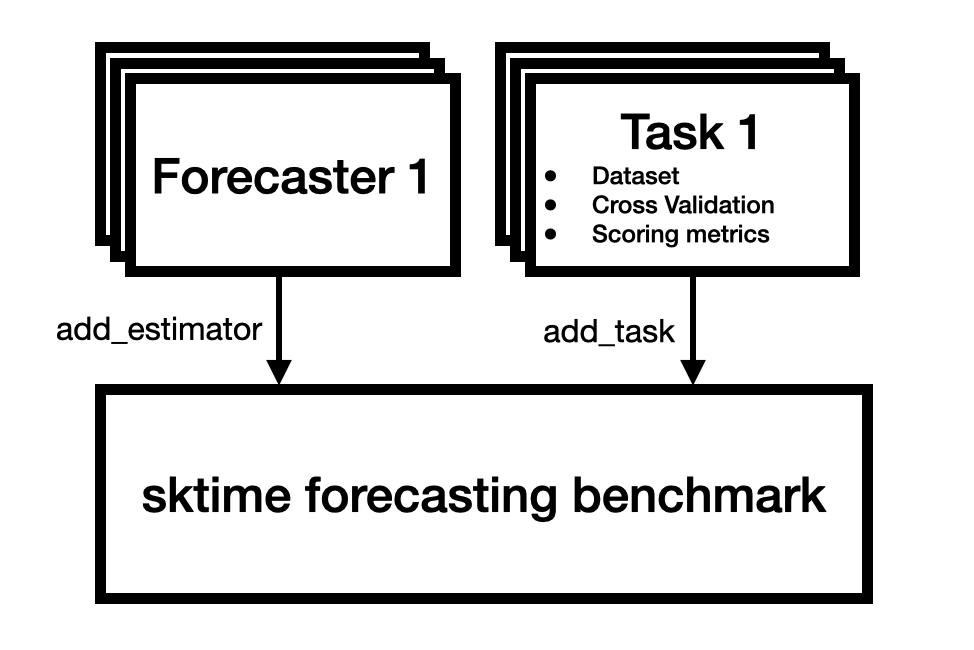
\includegraphics[width=.5\textwidth]{Figures/evaluationFramework.png}
    \caption{Caption}
    \label{fig:enter-label}
\end{figure}

\subsection{Prior work}

Design-wise, the first-order specification language, with relevant object orientation patterns, have been pioneered by scikit-learn in python (cite), mlr (cite), and Weka (cite). For a detailed of design patterns in AI framework packages, and innovations in \texttt{sktime}, see (patterns paper).

Specific \texttt{sktime} contributions are: forecasting interfaces, including probabilistic forecasters; metrics interface for probabilistic metrics; reproducibility patterns and APIs; meta-algorithms and inhomogeneous API composition, e.g., adding probability prediction mode.

Similar patterns specific to forecasting are found in the R/fable package (cite), which adapted, or rediscovered, some of the above later.


\section{Experiment: Algorithms} \label{methods}

In this section, we describe the forecasting algorithms used in the experiments. The methods combine traditional forecasting models with uncertainty estimation wrappers.

We stress that the study is relatively small and serves primarily as an illustration of benchmarking and model specification capabilities of \texttt{sktime} - and as an invitation to the scientific python community to engage and contribute to a more systematic study with reproducible specifications.

From a software perspective, is also worth noting that \texttt{sktime} provides a unified interface across multiple packages in the time series ecosystem in which time series algorithms are located:

\begin{itemize}
    \item \textbf{tsbootstrap} (cite): A library for time series bootstrapping methods. Second party package integrated with \texttt{sktime}.
    \item \textbf{statsforecast} (cite): A library for statistical and econometric forecasting methods. Location of the Auto-Theta algorithm, interfaced third party.
    \item \textbf{sktime} (cite zenodo): contains multiple native implementations: naive methods, all probability wrappers, and pipeline composition.
    \item \textbf{statsmodels} (cite): A foundational library for statistical methods. Location of the deseasonalizer, and indirectly used through various statistical primitives called from \texttt{tsbootstrap}, \texttt{sktime}, and \texttt{statsforecast}.
\end{itemize}

The hybrid use of \texttt{sktime} as a framework covering first party (itself), second (\texttt{tsbootstrap}), and third party (\texttt{statsmodels}, \texttt{statsforecast}) locations, should be noted.

Credit hence also goes to the maintainers and implementers of the cited locations.

\subsection{Forecasting Pipeline}
Every forecaster is wrapped in Differencer and a Deseasonalizer as preprocessing steps to improve stationarity. We use both preprocessors since some of the forecasters require that the time series are stationary and non-seasonal.

\begin{itemize}
    \item \texttt{Differencer}: This component, with default settings, computes first differences, which are inverted after forecast by cumulative summing.
    \item \texttt{Deseasonalizer(sp=data\_sp):} naive deseasonalizer from \texttt{statsmodels}. Description from source package: "first estimates the trend by applying a convolution filter to the data. The trend is then removed from the series and the average of this de-trended series for each period is the returned seasonal component.". After forecast, the estimated seasonal component is added back.
\end{itemize}

All forecasters are point forecasters, composed with one of the considered probabilistic wrappers. These wrappers are applied to the pre-processed time series to generate prediction intervals and probabilistic forecasts.

\begin{figure}
    \centering
    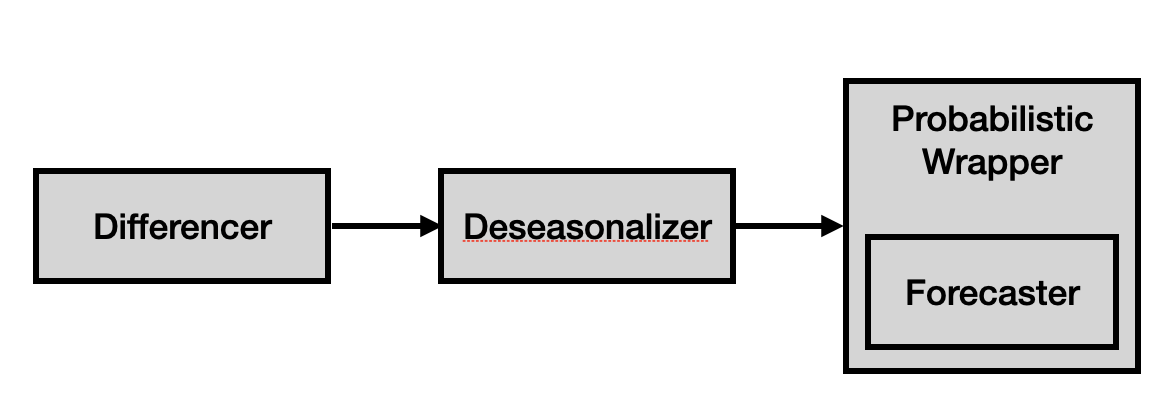
\includegraphics[width=\textwidth]{Figures/Pipeline.png}
    \caption{The forecasting pipeline used for all the forecasters}
    \label{fig:pipeline}
\end{figure}

The partial pipeline specification, illustrated in Figure \ref{fig:pipeline}, is

\begin{verbatim}
Differencer() * Deseasonalizer(sp=data\_sp) * wrapper(forecaster)
\end{verbatim}

where variable parts are \texttt{wrapper}, \texttt{forecaster}, and \texttt{data\_sp}. These are varied across different choices as described below.

We call the \texttt{forecaster} below "component model".

\subsection{Component forecasting models}

The component models used in this study are:

\begin{itemize}
    
    \item \texttt{NaiveForecaster(strategy, sp)} - Naive forecasters make forecasts using simple heuristics. Thet \texttt{strategy} parameter allows to select the type of algorithm
    \begin{itemize}
        \item The \texttt{mean} method uses the mean of the last \(N\) values that fit the same seasonality as the value to be forecast. Formally:
        \begin{equation}
            \hat{y}_t = \frac{1}{N} \sum_{i=1}^N y_{t-s \cdot i},
        \end{equation}
        where \(s\) is the seasonal length.
        \item The \texttt{last} method uses the last observed value considering the selected seasonal length. Formally:
        \begin{equation}
            \hat{y}_t = y_{t-s},
        \end{equation}
        where \(s\) is the selected seasonal length.
        \item The \texttt{drift} method fits a line between the first value and the last value of the considered window and projects it forward. Formally:
        \begin{equation}
            \hat{y}_t = y_{t-1} + \frac{y_{t-1} - y_1}{n-1} \cdot (t - (n-1)),
        \end{equation}
        where \(n\) is the number of points in the window.
    \end{itemize}

    \item \texttt{StatsForecastAutoTheta(sp)} - The AutoTheta method is a variant of the Theta model \cite{Assimakopoulos2000} with automated parameter tuning, from the \texttt{statsmodels} library.
    
\end{itemize}


\subsection{Probabilistic Wrappers}
The below components were used as probabilistic wrappers:


\begin{itemize}
    
    \item \texttt{ConformalIntervals(forecaster, strategy)} - "conformal prediction" is a theoretical framework adjacent to bootstrap and jackknife techniques to produce non-parametric prediction intervals. The \texttt{sktime} estimator implements variants of the method that are selectec by the \texttt{strategy} parameter: \textbf{Empirical} and \textbf{Empirical Residual} are non-conformal, naive predictions using training quantiles, with "residual" using symmetrized residuals method. \textbf{Conformal} implements the method of \cite{Stankeviciute2021}, \textbf{Conformal Bonferroni} additionally applies the Bonferroni correction described in the reference.

    \item \texttt{BaggingForecaster(bootstrap\_transformer, forecaster)} - probabilistic forecasts can be obtained from bootstrapping time series and aggregating the bootstrap forecasts, see \cite{hyndman2018,bergmeir2016}. The \texttt{BaggingForecaster} takes as parameter a bootstrap algorithm \texttt{bootstrap\_transformer}, also a first-class object in \texttt{sktime} (transformation). In the study, various bootstrap algorithms are applied, with their own parameters, as listed in the next section.

    \item \texttt{NaiveVariance(forecaster)} - The naive variance wrapper uses a sliding window to compute backtesting residuals. These residuals are then aggregated by forecasting horizon to a variance estimate, used in a normal prediction where mean is obtained from the wrapped forecaster, and variance from the pooled backtesting estimate.

    \item \texttt{SquaringResiduals(forecaster, residual\_forecaster)} - the "squaring residuals" strategy takes \texttt{forecaster} to obtain backtesting residuals on the training set, squares them, and fits the \texttt{residual\_forecaster} to the squared residuals. Forecasts of \texttt{residual\_forecaster} are then used as variance predictions, with mean predictions from \texttt{forecaster}, to obtain a normal distributed forecast. In the study, \texttt{residual\_forecaster} is always \texttt{NaiveForcaster(strategy="last")}.

\end{itemize}


\subsection{Bootstrapping Techniques}

Bootstrapping methods generate multiple resampled datasets from the original time series data, this can be used as part of wrappers to estimate prediction intervals or predictive distributions.

In the study, bootstrap algorithms from \texttt{tsbootstrap} are used, an \texttt{sktime} and \texttt{sklearn} compatible framework library dedicated to time series bootstrap algorithms. \texttt{sktime} adapts bootstrap algorithms to time series transformations via the \texttt{TSBootstrapAdapter}, with \texttt{bootstrap\_transformer} in \texttt{BaggingForecaster} taking the form of \texttt{TSBootstrapAdapter(bootstrap)} where \texttt{bootstrap} is any of the algorithms below.

\begin{itemize}
    
    \item \texttt{MovingBlockBootstrap} -
    The MBB method involves dividing the time series data into overlapping blocks of a fixed size and resampling these blocks to create new datasets. The block size is chosen to capture the dependence structure in the data. 

    \item \texttt{BlockDistributionBootstrap} -
    The Block Distribution Bootstrap generates bootstrapped samples by fitting a distribution to the residuals of a model and then generating new residuals from the fitted distribution. The new residuals are added to the fitted values to create the bootstrapped samples. This method assumes that the residuals follow a specific distribution, such as Gaussian or Poisson. The blocked version handles dependencies by resampling blocks of residuals.

    \item \texttt{BlockResidualBootstrap} -
    The Block Residual Bootstrap is designed for time series data where a model is fit to the data, and the residuals (the difference between the observed and predicted data) are bootstrapped. This method is particularly useful when a good model fit is available for the data. The bootstrapped samples are created by adding the bootstrapped residuals to the model's fitted values.

    \item \texttt{BlockStatisticPreservingBootstrap} -
    The Block Statistic-Preserving Bootstrap generates bootstrapped time series data while preserving a specific statistic of the original data. This method is beneficial when it is important to maintain the original data's characteristics in the bootstrapped samples. The blocked version handles dependencies by resampling blocks of data while ensuring that the preserved statistic remains consistent.

\end{itemize}

In the study, these bootstrapping techniques are used to estimate the distribution of forecasts and generate robust prediction intervals and predictive distributions, as part of the \texttt{BaggingForecaster}.


\subsection{Evaluation Metrics}
Performances are evaluated using the following metrics:

\subsubsection{Continuous Ranked Probability Score (CRPS)}
CRPS \cite{matheson1976} measures the accuracy of probabilistic forecasts by comparing the predicted distribution to the observed values. The CRPS for a forecast distribution \( F \) and an observation \( y \) is defined as:
\begin{equation}
\text{CRPS}(F, y) = \int_{-\infty}^\infty \left[ F(x) - \mathbf{1}(x \ge y) \right]^2 dx,
\end{equation}
where \( \mathbf{1} \) is the indicator function.

\subsubsection{Pinball Loss}
Pinball Loss evaluates the accuracy of quantile forecasts by penalizing deviations from the true values based on specified quantiles. For a quantile forecast \( \hat{q}_\tau \) at level \( \tau \) and an observation \( y \), the Pinball Loss is defined as:
\begin{equation}
\text{Pinball Loss}(\hat{q}_\tau, y) = \begin{cases}
\tau (y - \hat{q}_\tau), & \text{if } y \ge \hat{q}_\tau, \\
(1 - \tau) (\hat{q}_\tau - y), & \text{otherwise}.
\end{cases}
\end{equation}

\subsubsection{Calibration}
Calibration assesses how well the prediction intervals capture the true values. Well-calibrated intervals should contain the observed values with the specified probability. To assess the calibration quantitatively, we use the Area Under the Calibration curve (AUCalibration):
\begin{equation}
AUC = \frac{1}{N} \sum_{i=1}^N c_{(i)} - \frac{i}{N},
\end{equation}
where \(c_{(i)}\) represents the calibration value at the \(i\)-th point, and \(N\) is the total number of points.

\subsubsection{Sharpness}
Sharpness measures the concentration of the prediction intervals. More concentrated intervals indicate higher confidence in the forecasts. Sharpness is desirable because it indicates precise predictions.

\subsubsection{Empirical Coverage}
Empirical coverage measures how much of the observations are within the predicted interval. It is computed as the proportion of observations that fall within the prediction intervals, providing a direct measure of the reliability of the intervals.

\subsubsection{Runtime}
Besides metrics that assess the quality of the forecast, we also consider runtime to estimate the feasibility of the examined approaches. Runtime measures the computational efficiency of the forecasting methods, which is crucial for practical applications.

\section{Datasets} \label{datasets}
We conduct our experiments on several diverse time series datasets to evaluate the performance of our forecasting methods and probabilistic wrappers. The datasets used in this study are as follows:

\subsubsection{Australian Electricity Demand}
This dataset consists of half-hourly electricity demand data for five different series in Australia. It provides a comprehensive view of electricity consumption patterns and is useful for evaluating the performance of forecasting models on high-frequency data.

\subsubsection{Sunspot Activity}
The sunspot dataset contains weekly observations of sunspot numbers. Sunspot activity is a well-known time series with long-term periodic patterns, making it an ideal candidate for testing the robustness of our forecasting methods.

\subsubsection{US Births}
This dataset records the daily number of births in the United States. It is a univariate time series with a clear seasonal pattern, suitable for assessing the performance of our models on daily data.

For all datasets, we preprocess the data to handle missing values and ensure consistency. We also apply differencing and deseasonalization techniques to improve the performance of our forecasting models, except for automatic models like ARIMA and BATS.

These datasets offer a diverse range of time series characteristics, allowing us to thoroughly evaluate the effectiveness of combining bootstrapping techniques with traditional forecasting methods.

\begin{table}[h]
    \centering
    \footnotesize

    \caption{Evaluation Splits. Used Splitter: Sliding Window Splitter}
    \label{tab:evaluation_splits}
    \begin{tabularx}{\textwidth}{X|X|X|X|X|X|X}
         \toprule
        Dataset & Forecast Horizon & Step Width & Window Size & Cutout Period & Number of Folds & Seasonal Length \\ \midrule
        Australian Electricity Demand & 48 & 1440 & 1440 & Last Year & 12 & 48 \\ 
        Sunspot Activity & 28 & 395 & 365 & Last 40 Years & 12 & 1\\
        US Births & 28 & 395 & 365 & Whole Time Series & 12 & 1 \\
        \bottomrule
    \end{tabularx}
\end{table}

\section{Experiments} \label{experiments}
In this section, we describe the experimental setup, including the hardware and software used, the datasets, the evaluation metrics, and the experimental procedures. We explain how the experiments were designed to compare the performance of different forecasting methods.



\subsection{Software Setup}

Todo: Mention versions and location of pip freeze for reproducibility.

\subsection{Experimental Setup}
To perform the benchmarking study, we use the framework described in Section~\ref{methods}. The benchmarking compares different probabilistic wrappers on different datasets and with different forecasters regarding CRPS, Pinball Loss, AUCalibration, and Runtime. 

To enable easy replication of the experiments, we provide for each used forecaster, and wrapper the hyperparameters by providing the used python object instantiation in Table~\ref{tab:hyperparams}. These hyperparameter depend on the dataset, especially, the seasonal periodicity (sp) is chosen based on the dataset. This parameter as well as the other dataset related parameter required to instantiate the cross validation used for the evaluation are described in Table~\ref{tab:evaluation_splits}.

% \begin{itemize}
%     \item \textbf{Data Preprocessing:} We preprocess the datasets by handling missing values, normalizing the data, and splitting it into training and test sets.
%     \item \textbf{Model Training:} We train each forecasting model on the training set. For ARIMA models, we use the AutoARIMA function to automatically select the best hyperparameters. For naive forecasters, we use the mean, last, and drift methods as described earlier.
%     \item \textbf{Bootstrapping:} We apply the Moving Block Bootstrap (MBB) technique, as well as other blocked bootstrapping techniques, to generate multiple resampled datasets from the training data.
%     \item \textbf{Prediction Interval Generation:} We use the bootstrapped datasets to generate prediction intervals for each forecasting model.
%     \item \textbf{Evaluation:} We evaluate the performance of the forecasting models and probabilistic wrappers using the metrics described in the Methodology section.
% \end{itemize}

\begin{table}[]
    \centering    \caption{
    In sktime, the hyperparameters of the methods are determined during initialisation of the estimator. Thus, we provide the initialisation code. \\
    Some of the parameters are determined by the used dataset: sp is 48 for the Autralian Electricity Dataset and 1 for the other. The sample\_freq is 0.005 for the Australian Electricity Dataset and 0.1 for the other.\\}
    \label{tab:hyperparams}
    \footnotesize
    \begin{tabular}{p{2.5cm}p{4cm}|p{7.5cm}}
    \toprule  
         Role & Name &  Hyperparameters \\ \midrule
         Base Forecaster & Naive last &  \texttt{NaiveForecaster(strategy="last", sp=sp)}\\
         Base Forecaster &  Naive mean &  \texttt{NaiveForecaster(strategy="mean", sp=sp)}\\
         Base Forecaster & Naive drift &  \texttt{NaiveForecaster(strategy="drift", sp=sp)}\\ 
         Base Forecaster & Theta &   \texttt{StatsForecastAutoTheta(season\_length=sp)} \\ \midrule
         Wrapper & CI Empirical & \texttt{ConformalIntervals(forecaster, sample\_frac=sample\_frac)} \\
         Wrapper & CI Empirical residuals & \texttt{ConformalIntervals(forecaster, sample\_frac=sample\_frac, method="empirical\_residual")} \\
         Wrapper & CI Conformal & \texttt{ConformalIntervals(forecaster, sample\_frac=sample\_frac, method="conformal")} \\
         Wrapper & CI Bonferroni & \texttt{ConformalIntervals(forecaster, sample\_frac=sample\_frac, method="conformal\_bonferroni")} \\
         Wrapper & BaggingForecaster & \texttt{BaggingForecaster(ts\_bootstrap\_adapter, forecaster))} \\
         Wrapper & Naive Variance & \texttt{NaiveVariance(forecaster, initial\_window=14*sp))}\\
         Wrapper & Squaring Residuals & \texttt{SquaringResiduals(forecaster, initial\_window=14*sp))}  \\ \midrule
         Forecasting Pipeline & Pipeline & \texttt{Differencer(1) * Deaseasonalizer(sp=sp) * Wrapper} \\ \midrule
        
         ts\_bootstrap\_adapter & TSBootstrapAdapter & \texttt{TSBootstrapAdapter(tsbootsrap)} \\
         %Differencer& Differencer &  \\
         %Deseasonalizer & Deseasonalizer &  \\ 
         \midrule
 
         tsbootstrap & Moving Block Bootstrap & \texttt{MovingBlockBootstrap()} \\
         tsbootstrap & Block Residual Bootstrap & \texttt{BlockDistributionBootstrap()} \\
         tsbootstrap & Block Statistic Preserving Bootstrap & \texttt{BlockStatisticPreservingBootstrap()} \\
         tsbootstrap & Block Distribution Bootstrap & \texttt{BlockDistributionBootstrap()}\\

         \bottomrule
         
    \end{tabular}
\end{table}

% \subsection{Evaluation Metrics}
% The evaluation metrics used in this study include Continuous Ranked Probability Score (CRPS), Pinball Loss, Calibration, Sharpness, Empirical Coverage, and Runtime. These metrics provide a comprehensive assessment of the accuracy, reliability, and computational efficiency of the probabilistic forecasts.

% \subsection{Experimental Procedure}
% We conduct experiments on each dataset by following the experimental setup described above. For each dataset, we train the forecasting models on the training set and generate prediction intervals using the bootstrapped datasets. We then evaluate the performance of the models and probabilistic wrappers on the test set using the evaluation metrics.


\subsection{Results} \label{results}
In this section, we present the results of our experiments. We evaluate the performance of the forecasting methods combined with probabilistic wrappers on the datasets described in Section \ref{datasets}. 
%Our primary focus is on the accuracy and reliability of the prediction intervals generated by these methods.
To increase the conciseness, we calculated the rank of each probabilistic wrapper for each combination of forecaster, metric, and dataset. Afterwards, for each metric, probabilistic wrapper and dataset, we have calculated the average across all forecasters and time series. In the following, we present the results for each dataset separately. 


\subsubsection{Performance on Australian Electricity Demand}
The results for the Australian electricity demand dataset are summarized in Table \ref{table:aus_elec_results}. We compare the performance of different forecasting models and probabilistic wrappers using the evaluation metrics described in Section \ref{methods}. 

The ranked based evaluation show that diverse results regarding the different metrics. E.g. while CI Empirical Residual performs best on CRPS, it is only mediocre regarding the Pinball Loss and the AUCalibration. On PinballLoss, the best method is CI Empirical and on AUCalibration, it is Squaring Residuals. Regarding the runtime, the fastest method is the fallback probabilistic prediction of the base forecaster. The slowest methods are NaiveVariance and SquaringResiduals. \textcolor{red}{Since easy optimisations are not implemented..} Furthermore, it seems that the ConformalIntervals are slightly faster than the BasggingForecasters \textcolor{red}{Depends heavily on chosen hyperparameters..}.

\begin{table}[h]
    \centering
    \caption{Performance of forecasting methods on the Australian electricity demand dataset}
    \label{table:aus_elec_results}
\begin{tabular}{lrrrr}
\toprule
Wrapper & CRPS & Pinball Loss & AUCalibration & Runtime \\
\midrule
Fallback & 9.45 & 9.66 & 5.61 & 1.00 \\
Naive Variance & 7.75 & 7.20 & 7.15 & 10.00 \\
Squaring Residuals & 7.45 & 6.20 & 5.05 & 11.00 \\
Block Distribution Bootstrap & 4.08 & 3.15 & 6.82 & 7.83 \\
Block Residual Bootstrap & 4.30 & 5.58 & 5.84 & 8.32 \\
Block Statistic Preserving Bootstrap & 4.25 & 5.87 & 6.15 & 7.29 \\
Moving Block Bootstrap & 6.12 & 6.51 & 4.26 & 6.00 \\
CI Conformal & 5.75 & 5.40 & 5.69 & 3.92 \\
CI Empirical & 3.79 & 2.63 & 6.97 & 3.30 \\
CI Empirical Residual & 2.37 & 5.42 & 5.35 & 3.49 \\
CI Bonferroni  & 10.50 & 8.05 & 6.70 & 3.70 \\
\bottomrule
\end{tabular}

\end{table}

\subsubsection{Performance on Sunspot Activity}
Table \ref{table:sunspot_results} shows the performance of our methods on the sunspot activity dataset. The long-term periodic patterns in this dataset provide a challenging test for our forecasting models.

The ranked based evaluation show that BaggingForecaster with the Block Distribution Bootstrap scores clearly best regarding the CRPS and Pinball Loss, and AUCalibration. Regarding the runtime, the fastest method is the fallback probabilistic prediction of the base forecaster. The slowest methods are NaiveVariance and SquaringResiduals. 
\textcolor{red}{Since easy optimisations are not implemented..}Furthermore, it seems that the ConformalIntervals are slightly faster than the BasggingForecasters \textcolor{red}{Depends heavily on chosen hyperparameters..}. 
\begin{table}[h]
    \centering
    \caption{Performance of forecasting methods on the sunspot activity dataset}
    \label{table:sunspot_results}
\begin{tabular}{lrrrr}
\toprule
Wrapper & CRPS & PinballLoss & AUCalibration & Runtime \\
\midrule
Fallback & 9.00 & 7.25 & 9.50 & 1.00 \\
Naive Variance & 6.50 & 6.25 & 7.75 & 10.00 \\
Squaring Residuals & 8.00 & 8.00 & 4.75 & 11.00 \\
Block Distribution Bootstrap & 1.00 & 1.00 & 3.00 & 7.25 \\
Block Residual Bootstrap & 6.00 & 6.25 & 5.00 & 6.75 \\
Block Statistic Preserving Bootstrap & 5.50 & 7.00 & 2.50 & 6.25 \\
Moving Block Bootstrap & 5.75 & 5.75 & 7.50 & 5.00 \\
CI Conformal & 4.75 & 4.50 & 6.75 & 4.50 \\
CI Empirical & 5.50 & 4.00 & 7.25 & 4.50 \\
CI Empirical Residual & 3.50 & 8.00 & 6.25 & 4.25 \\
CI Bonferroni  & 10.50 & 8.00 & 5.75 & 5.50 \\
\bottomrule
\end{tabular}


\end{table}

\subsubsection{Performance on US Births}
The results for the US births dataset are presented in Table \ref{table:us_births_results}. This dataset, with its clear seasonal pattern, allows us to assess the models' ability to handle daily data.
The ranked based evaluation show that BaggingForecaster with the Block Distribution Bootstrap scores best regarding the CRPS and Pinball Loss. 
Regarding the AUCalibration, the best score is achieved by CI Conformal. Regarding the runtime, the fastest method is the fallback probabilistic prediction of the base forecaster. The slowest methods are NaiveVariance and SquaringResiduals. 
\textcolor{red}{Since easy optimisations are not implemented..}Furthermore, it seems that the ConformalIntervals are slightly faster than the BasggingForecasters \textcolor{red}{Depends heavily on chosen hyperparameters..}. 

\begin{table}[h]
    \centering
    \caption{Performance of forecasting methods on the US births dataset}
    \label{table:us_births_results}
\begin{tabular}{lrrrr}
\toprule
Wrapper & CRPS & PinballLoss & AUCalibration & Runtime \\
\midrule
Fallback & 9.25 & 9.50 & 7.88 & 1.00 \\
Naive Variance & 6.25 & 5.75 & 6.25 & 10.00 \\
Squaring Residuals & 9.50 & 8.50 & 6.50 & 11.00 \\
Block Distribution Bootstrap & 1.00 & 1.00 & 8.25 & 7.25 \\
Block Residual Bootstrap & 3.75 & 5.75 & 5.50 & 7.00 \\
Block Statistic Preserving Bootstrap & 5.50 & 6.00 & 7.38 & 6.25 \\
Moving Block Bootstrap & 5.75 & 5.25 & 5.12 & 4.75 \\
CI Conformal & 6.00 & 6.00 & 4.75 & 4.25 \\
CI Empirical & 5.50 & 4.50 & 4.88 & 4.75 \\
CI Empirical Residual & 3.00 & 6.00 & 5.00 & 5.25 \\
CI Bonferroni  & 10.50 & 7.75 & 4.50 & 4.50 \\
\bottomrule
\end{tabular}

\end{table}

\iffalse
\subsection{Visualizations of Results}
We provide visualizations of the prediction intervals generated by each forecasting model on the test set. Figures \ref{fig:arima}, \ref{fig:naive_mean}, \ref{fig:naive_last}, and \ref{fig:naive_drift} show the prediction intervals for the ARIMA, Naive Mean, Naive Last, and Naive Drift models, respectively.

\begin{figure}[h]
    \centering
    \includegraphics[width=\textwidth]{Figures/ARIMA_Prediction_Intervals.png}
    \caption{Prediction intervals generated by the ARIMA model}
    \label{fig:arima}
\end{figure}

\begin{figure}[h]
    \centering
    \includegraphics[width=\textwidth]{Figures/Naive_Mean_Prediction_Intervals.png}
    \caption{Prediction intervals generated by the Naive Mean model}
    \label{fig:naive_mean}
\end{figure}

\begin{figure}[h]
    \centering
    \includegraphics[width=\textwidth]{Figures/Naive_Last_Prediction_Intervals.png}
    \caption{Prediction intervals generated by the Naive Last model}
    \label{fig:naive_last}
\end{figure}

\begin{figure}[h]
    \centering
    \includegraphics[width=\textwidth]{Figures/Naive_Drift_Prediction_Intervals.png}
    \caption{Prediction intervals generated by the Naive Drift model}
    \label{fig:naive_drift}
\end{figure}
\fi

\section{Discussion and Conclusion} \label{conclusion}

Topics to discuss
\begin{itemize}
    \item Experiments show that the framework enables easy creation of benchmarking studies using sktime.
    \item The usage of two different systems show that the benchmark enables easily reproducible experiments.
    \item Regarding the results, a disclaimer is that we are haven't done a GridSearch on the best hyperparams for the Wrappers. Further Base Forecasters should be used in the future, More datasets etc.
    Furthermore, also regarding the runntime, the compute time of NaiveVariance and SquaringResiduals could be easily improved. 
    \item There exist further methods to make point forecasts probabilistic. E.g., using Generative Neural Networks, ...
\end{itemize}
%Our experiments demonstrate that combining bootstrapping techniques with traditional forecasting models significantly enhances the accuracy and reliability of prediction intervals. ARIMA models with bootstrapping consistently performed well across datasets, particularly in terms of CRPS and Calibration metrics. The BATS model showed strong performance on datasets with complex seasonal patterns, despite its longer runtimes. Reduction-based forecasters like XGBoost and Linear Regression also benefited from bootstrapping and conformal intervals, achieving reliable prediction intervals with good calibration and sharpness.

%These findings highlight the potential of bootstrapping techniques to make traditional forecasting methods more robust and reliable. Improved prediction intervals can inform decision-making processes, optimize operations, and enhance resource management in various domains. For example, accurate electricity demand forecasts can improve energy resource planning and distribution.

%The study also underscores the importance of considering runtime in practical applications. While bootstrapping increases computational time, the trade-off is justified by the improvements in forecast accuracy and reliability.

Several limitations need to be addressed in future research. The choice of block size in the Moving Block Bootstrap method significantly impacts results, necessitating the development of adaptive methods for optimal block size selection. Additionally, our experiments were limited to a few datasets. Future studies should evaluate the proposed methods on a wider range of datasets, including multivariate time series, and explore integrating generative networks for probabilistic forecasting.

In conclusion, combining bootstrapping techniques with traditional forecasting models enhances prediction robustness and reliability. This approach offers valuable insights and practical applications across various domains. Future research should continue to refine these methods, address current limitations, and explore new avenues for improvement, paving the way for more accurate and reliable time series predictions.


\bibliographystyle{alpha}
\bibliography{sample}

\section{Appendix}

\subsection{Hardware Setup}
We conduct our experiments on two different systems. The details of these systems are provided in Table \ref{tab:hardware_setup}.

\begin{table}[h]
    \centering
    \caption{Hardware Configuration}
    \label{tab:hardware_setup}
    \begin{tabular}{c|cc}\toprule
         & MacBook Air M2 & Sankalp's System  \\ \midrule
         GPUs & 8 & 12 \\
         RAM & 16 GB & 32 GB \\
         CPU Cores & 8 & 16 \\
        \bottomrule
    \end{tabular}
\end{table}

